
\subsection{Multi-Rate/stage}
\begin{frame}{Opbygning}{Multi-Rate/stage}
\begin{columns}
  \begin{column}{0.25\textwidth}
\begin{itemize}
\item Downsampling med faktor 2
\item 7 gange
\begin{itemize}
\item 48 kHz
\item 24 kHz
\item 12 kHz
\item ...
\item 375 Hz
\end{itemize}
\end{itemize}
  \end{column}
  \begin{column}{0.75\textwidth}
\begin{figure}
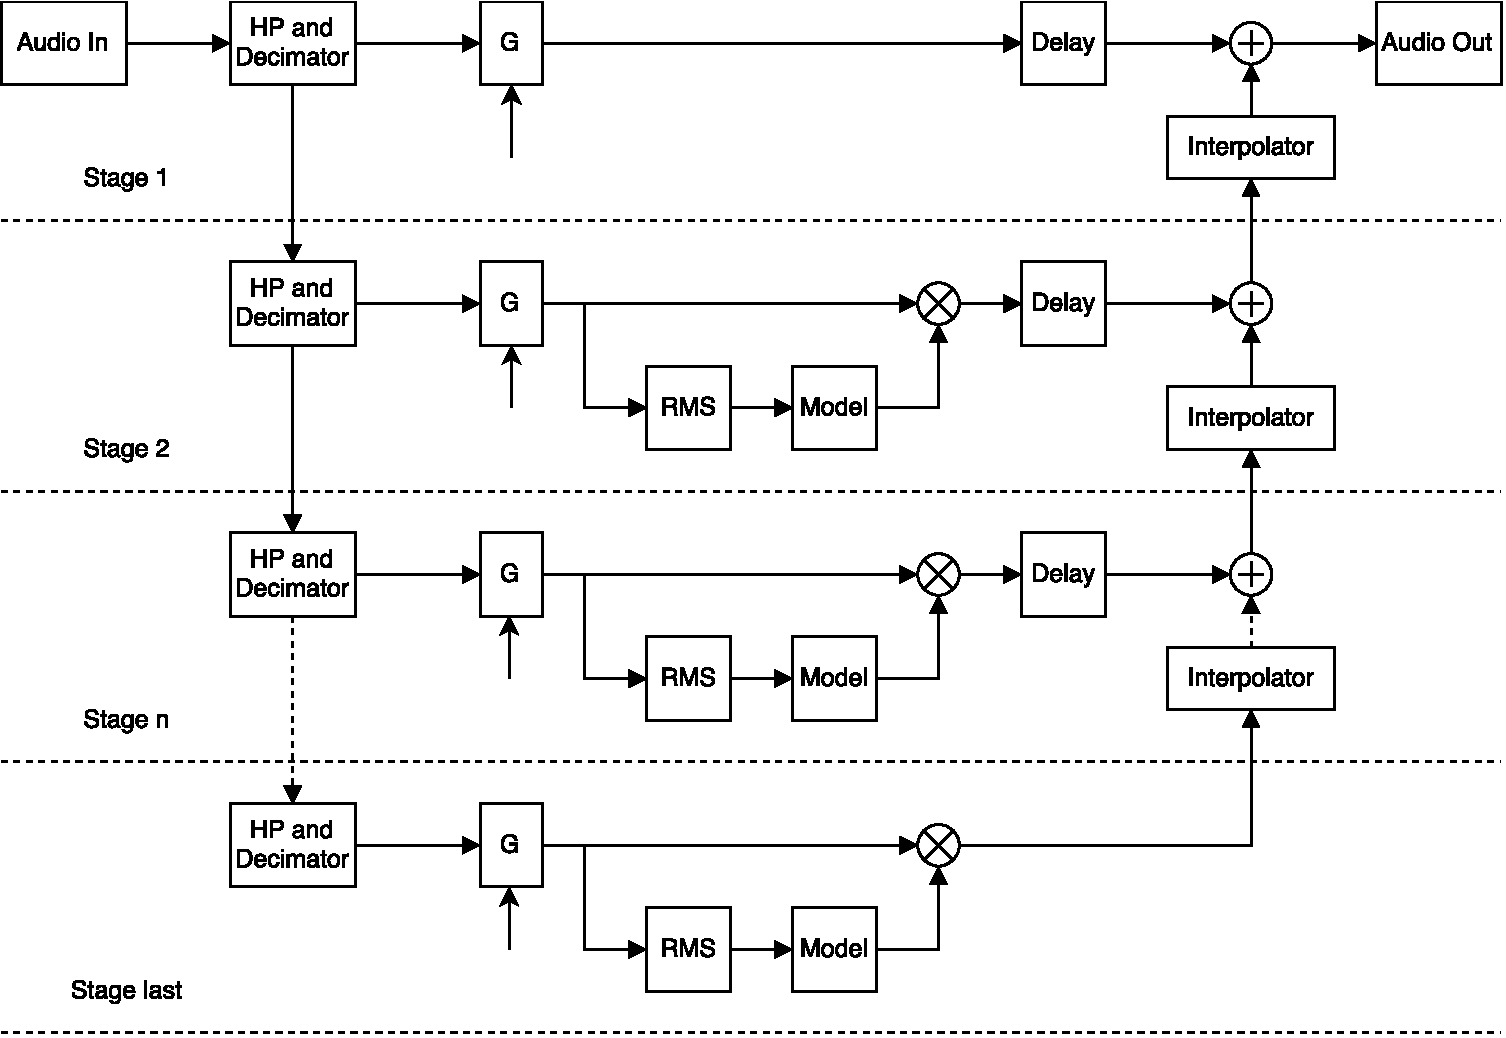
\includegraphics[width=\textwidth]{designRealBlock1}
\end{figure}
  \end{column}
\end{columns}
\end{frame}

\subsection{Decimation}
\begin{frame}{Opbygning}{Decimator}

\begin{columns}
  \begin{column}{0.4\textwidth}
  \textbf{Funktionalitet:}
\begin{itemize}
\item Lavpas filter til Anti-Aliasing
\item Spektral subtraktion til højpas filtrering 
\end{itemize}

\textbf{Krav:}
\begin{itemize}
\item Overholde IEC 6964 - Class 2
\item Lineær fase
\item 60 dB dæmpning ved $\frac{fs}{2L}$
\end{itemize}
  \end{column}
  \begin{column}{0.6\textwidth}
%\begin{figure}
%\centering
%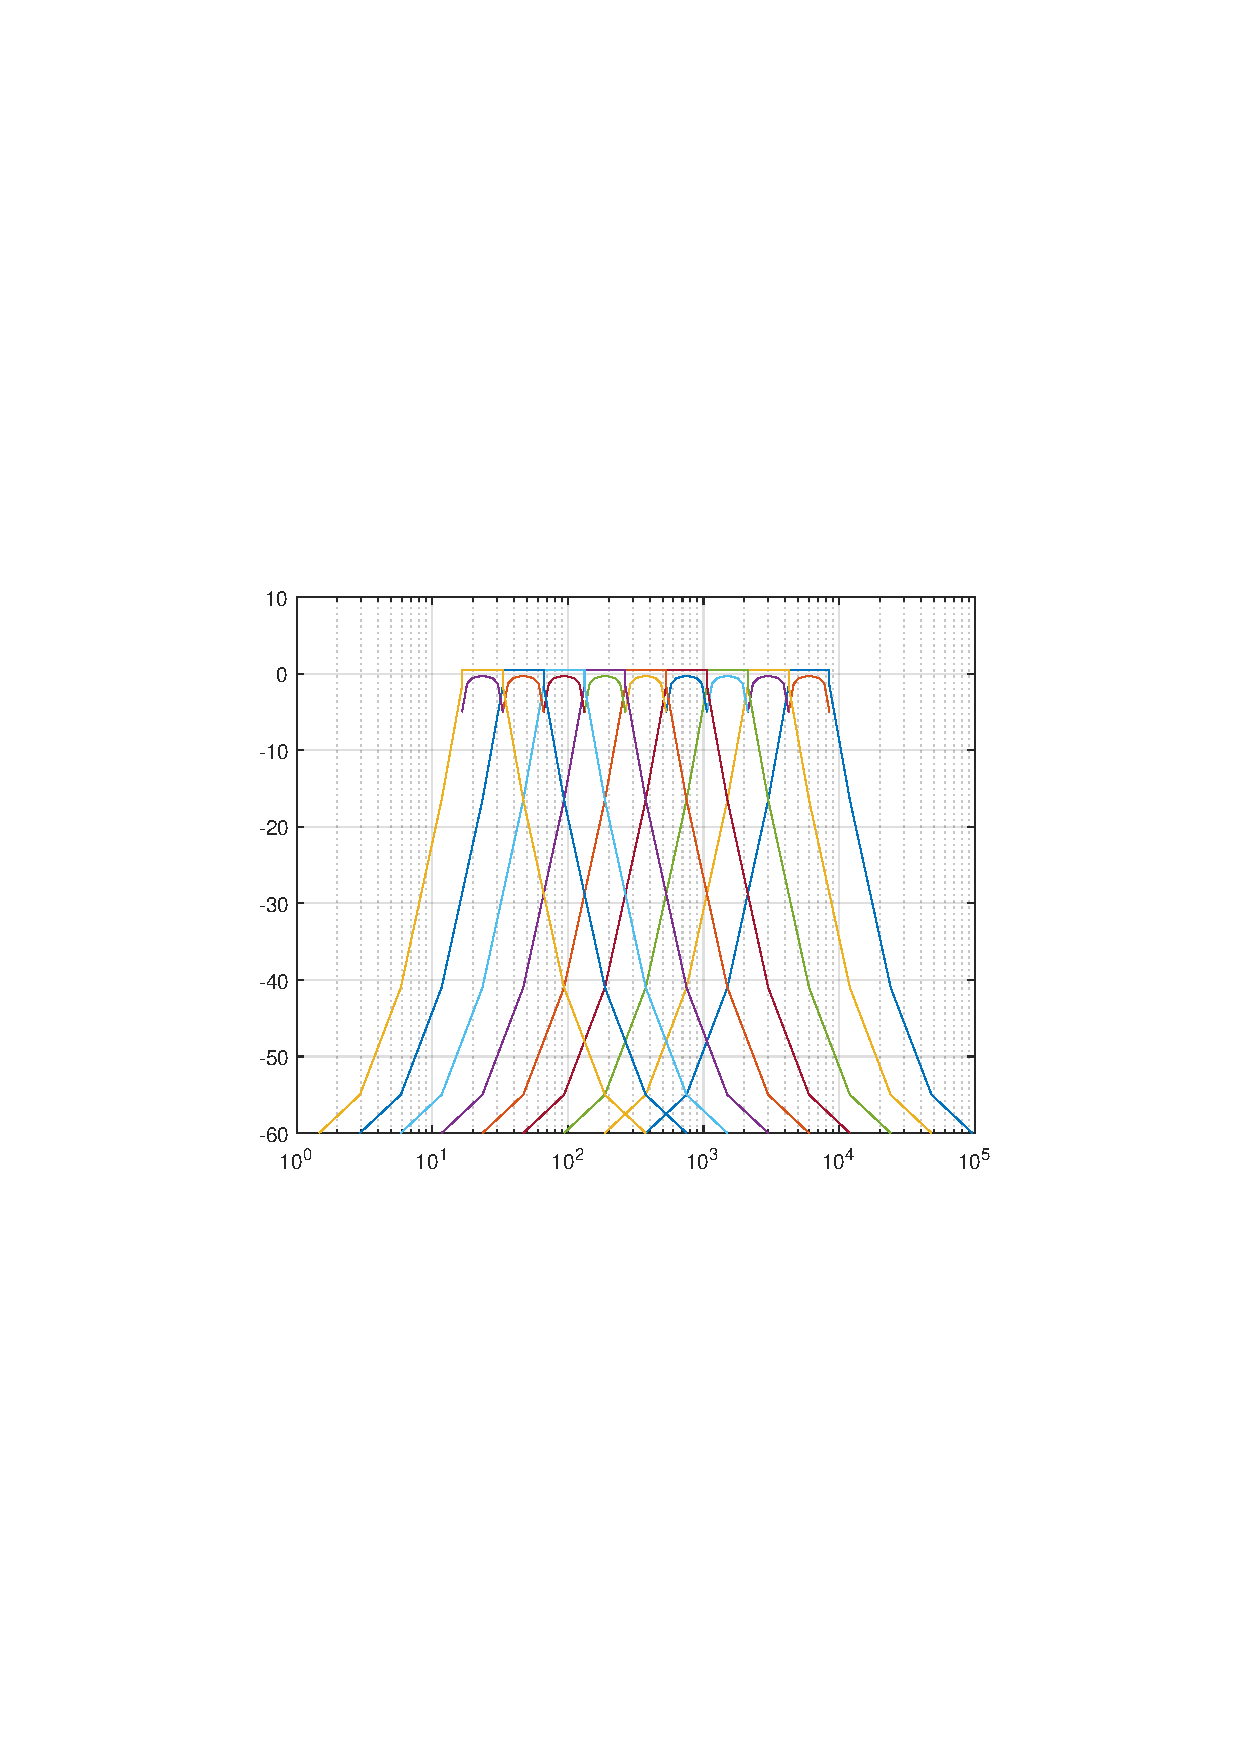
\includegraphics[width=0.5\textwidth]{Bands}
%\end{figure}
\begin{figure}
\centering
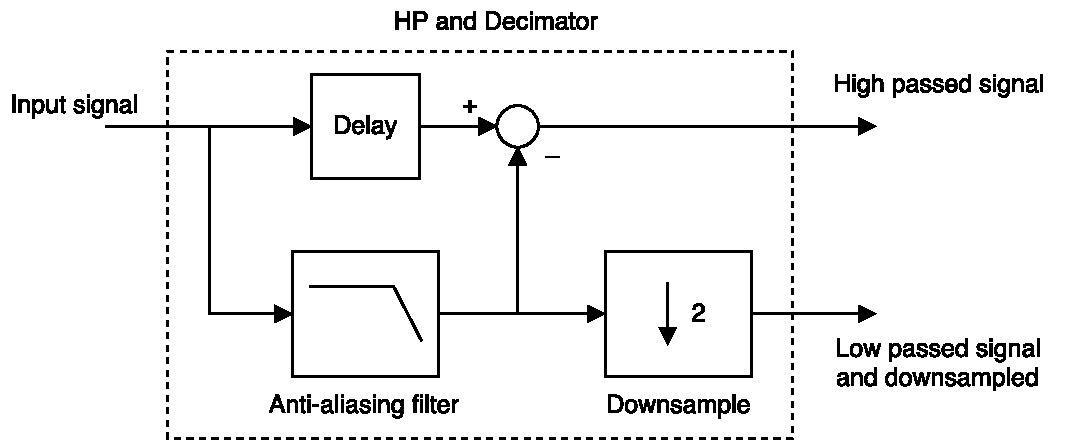
\includegraphics[width=0.9\textwidth]{designRealDecimator}
\end{figure}
  \end{column}
\end{columns}
\end{frame}

\begin{frame}{Opbygning}{IEC 6964 - Class 2}

\begin{columns}
  \begin{column}{0.4\textwidth}
\textbf{Krav:}
\begin{itemize}
\item[$\surd$] Overholde IEC 6964 - Class 2 
\item Lineær fase
\item 60 dB dæmpning ved $\frac{fs}{2L}$
\end{itemize}
  \end{column}
  \begin{column}{0.6\textwidth}


\begin{figure}
\centering
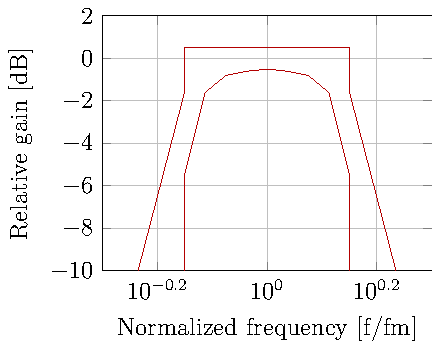
\includegraphics[width=0.5\textwidth]{Band1ReqZoom}
\end{figure}
\vspace*{-8mm} 
\begin{figure}
\centering
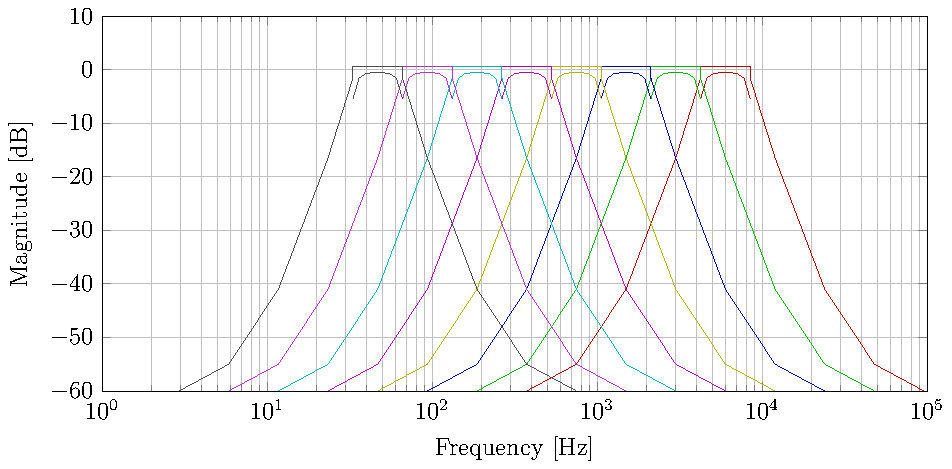
\includegraphics[width=0.9\textwidth]{allBands}
\end{figure}
  \end{column}
\end{columns}
\end{frame}


\begin{frame}{Opbygning}{Lineær fase \& 60 dB dæmpning ved $\frac{fs}{2L}$}

\begin{columns}
  \begin{column}{0.5\textwidth}
\textbf{Krav:}
\begin{itemize}
\item[$\surd$] Overholde IEC 6964 - Class 2
\item[$\surd$] Lineær fase
\begin{itemize}
\item[$\surd$] 50. Orden FIR
\item[$\surd$] Type 1
\begin{itemize}
\item[$\surd$] Symmetrisk
\item[$\surd$] Lige orden
\end{itemize}
\end{itemize}
\item[$\surd$] 60 dB dæmpning ved $\frac{fs}{2L}$
\begin{itemize}
\item $\omega_{\text{pass}}$= 0.125 $\frac{\pi rad}{sample} $ (3.000Hz)
\item $\omega_{\text{stop}}$= 0.271 $\frac{\pi rad}{sample} $ (6.500Hz)
\end{itemize}
\end{itemize}
\textbf{Metode brugt:}
\begin{itemize}
\item Kaiser Window method
\begin{itemize}
\item Effektivt design
\item Justerbar beta-værdi
\end{itemize}
\end{itemize}
  \end{column}
  \hspace*{-15mm}  
  \begin{column}{0.6\textwidth}

\begin{figure}
\centering
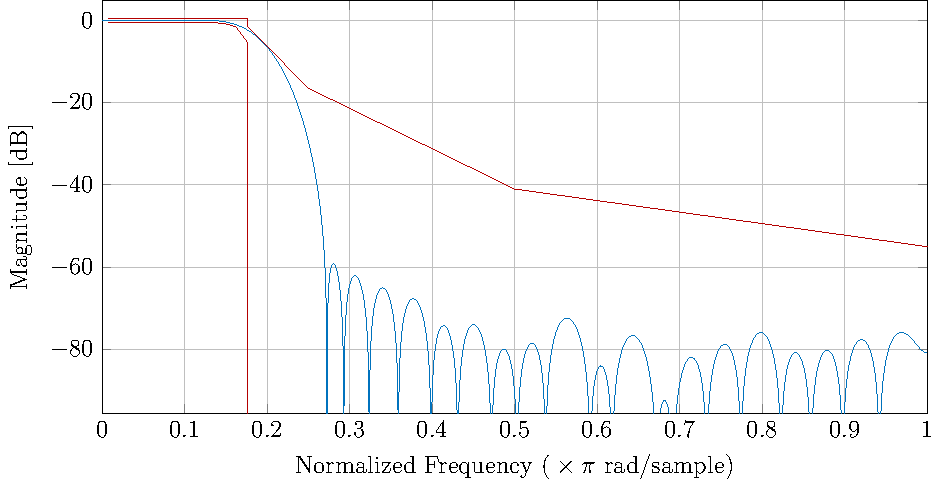
\includegraphics[width=0.9\textwidth]{Band1Filt}
\end{figure}
  \end{column}
\end{columns}
\end{frame}

%%%%%%%%%%%%%%%%%%%%%%%%%%%%%%%%%%%%%%%%%%%%%%%%%%%%%%%%%%%%%%%%%%%%%%%%%%%%
%%%%%%%%%%%%%%%%%%%%%%%%%%%%%%%%%%%%%%%%%%%%%%%%%%%%%%%%%%%%%%%%%%%%%%%%%%%%
%%%%%%%%%%%%%%%%%%%%%%%%%%%%%%%%%%%%%%%%%%%%%%%%%%%%%%%%%%%%%%%%%%%%%%%%%%%%


\subsection{RMS Limiter}
\begin{frame}{Opbygning}{RMS Limiter}
\begin{columns}
  \begin{column}{0.4\textwidth}
%\begin{figure}
%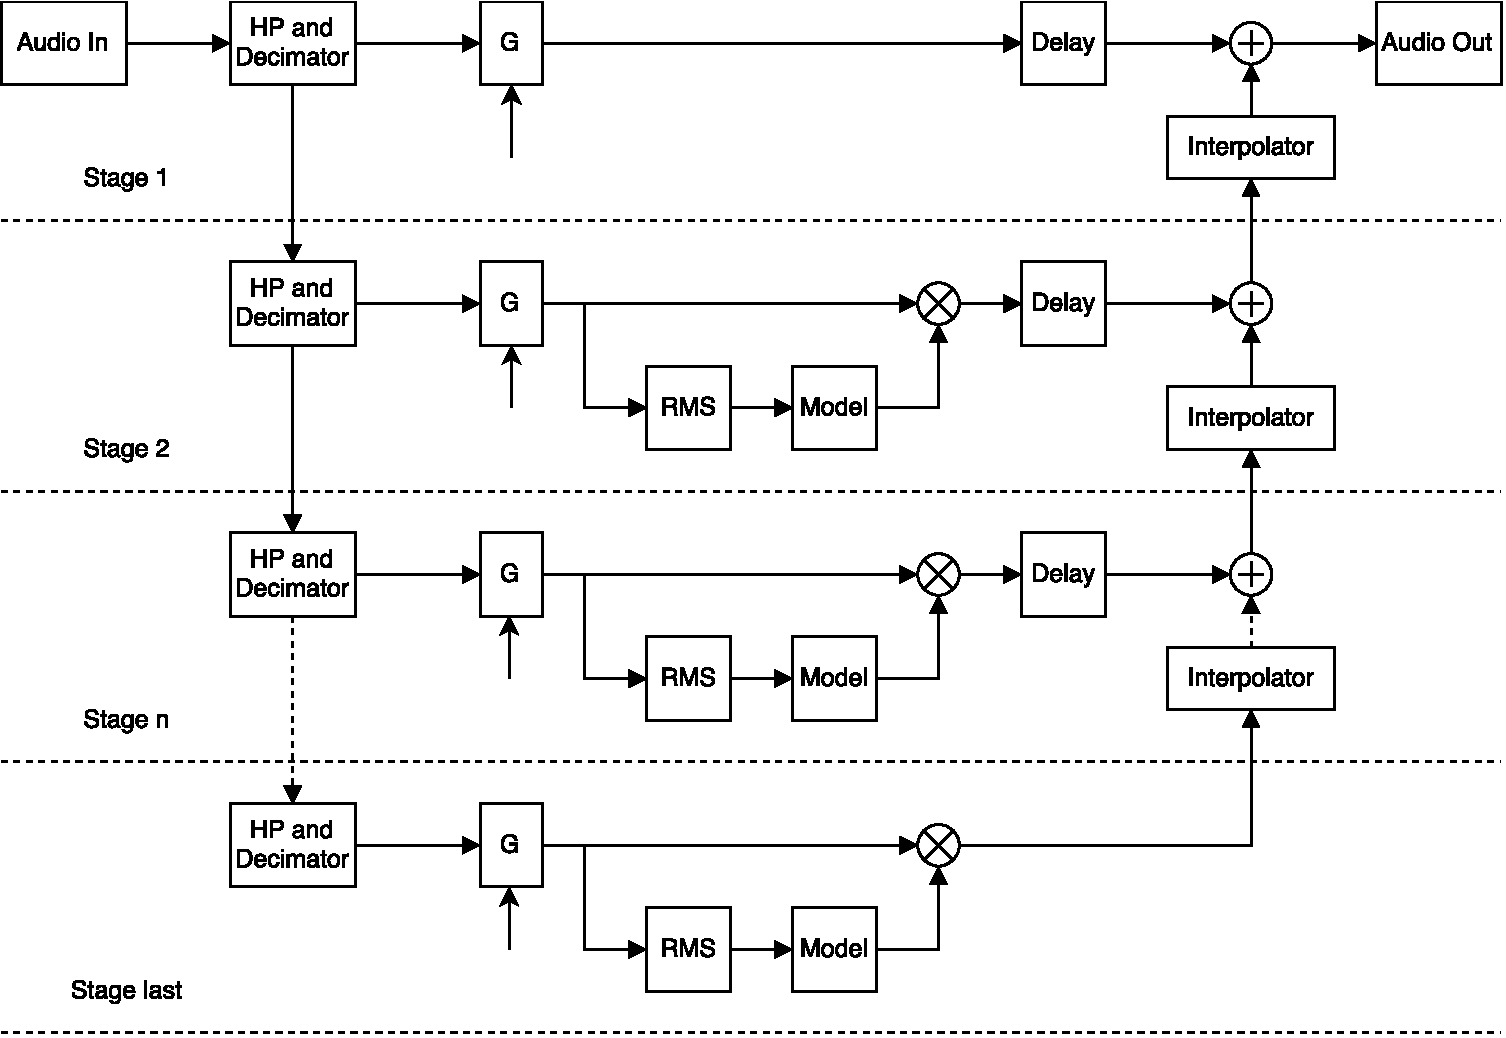
\includegraphics[width=0.9\textwidth]{designRealBlock1}
%\end{figure}
  \textbf{Funktionalitet:}
\begin{itemize}
\item Beregn RMS værdi i bånd
\item Bestem gain passende gain værdier
\item Påfører gain
\end{itemize}
\textbf{Krav:}
\begin{itemize}
\item Løbende Gennemsnit
\item \alert{Dæmpning til grænseværdi ved input på $\geq$ grænseværdien}
\item 0 s attack time
\item 5 s release time
\end{itemize}
  \end{column}

  \begin{column}{0.6\textwidth}
\begin{figure}
\centering
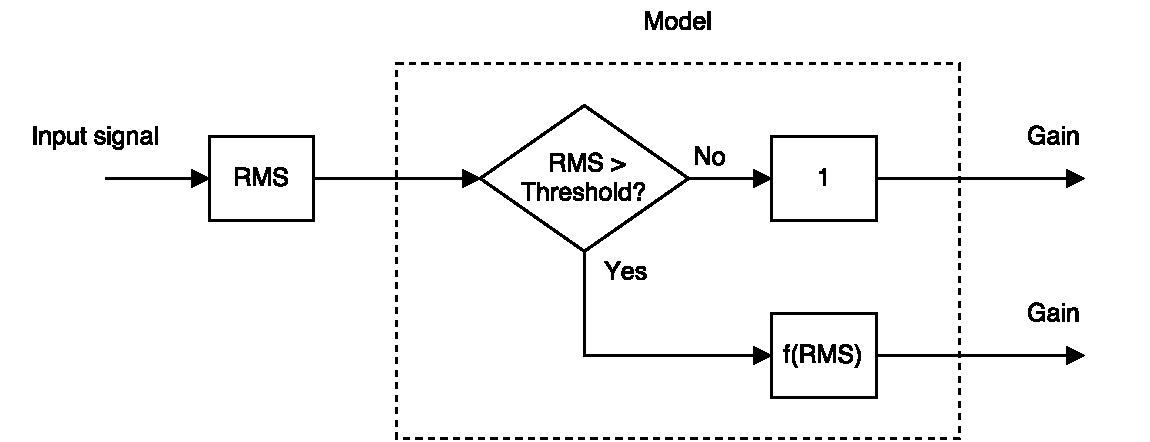
\includegraphics[width=\textwidth]{designRealRMS}
\end{figure}

%\begin{figure}
%	\centering
%	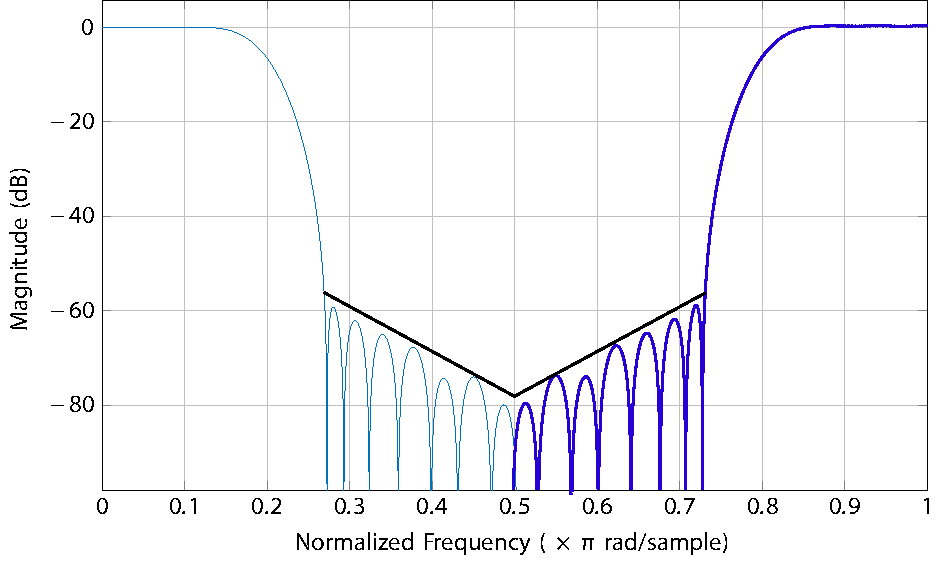
\includegraphics[width=0.8\textwidth]{DecIntCompMirror}
%\end{figure}

  \end{column}
\end{columns}
\end{frame}

\subsection{RMS Limiter}
\begin{frame}{Opbygning}{RMS Limiter}
\begin{columns}
  \begin{column}{0.4\textwidth}
%\begin{figure}
%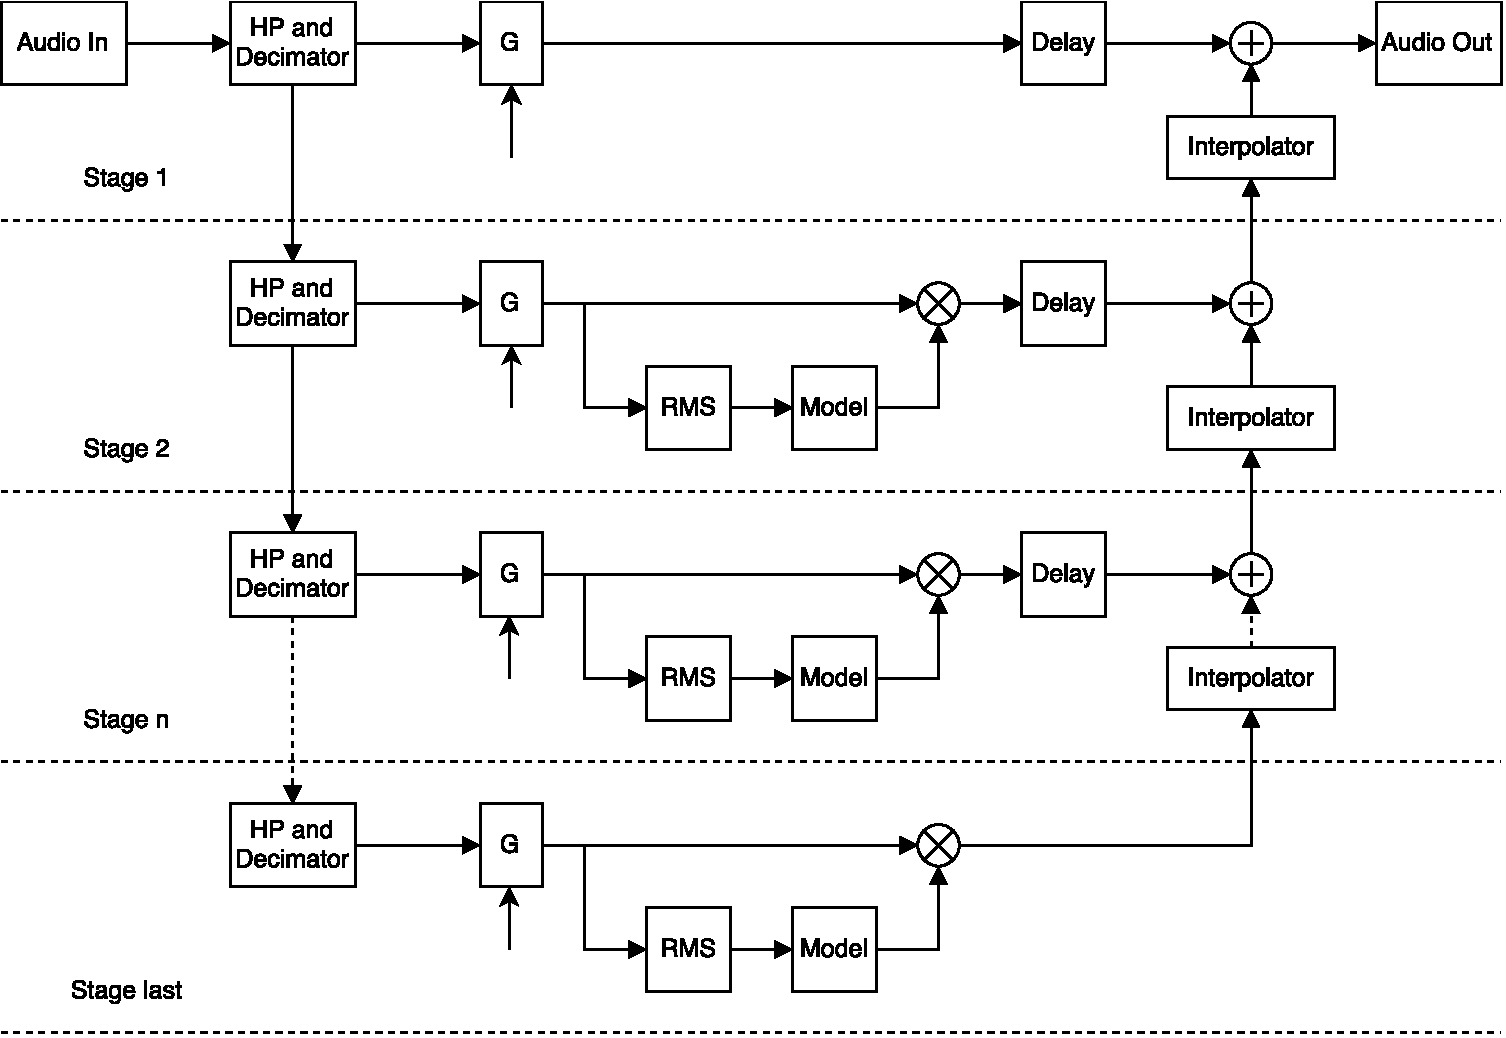
\includegraphics[width=0.9\textwidth]{designRealBlock1}
%\end{figure}
  \textbf{Funktionalitet:}
\begin{itemize}
\item Beregn RMS værdi i bånd
\item Bestem gain passende gain værdier
\item Påfører gain
\end{itemize}
\textbf{Krav:}
\begin{itemize}
\item Løbende Gennemsnit
\item \alert{Dæmpning til grænseværdi ved input på $\geq$ grænseværdien}
\item 0 s attack time
\item 5 s release time
\end{itemize}
  \end{column}

  \begin{column}{0.6\textwidth}
\begin{figure}
\centering
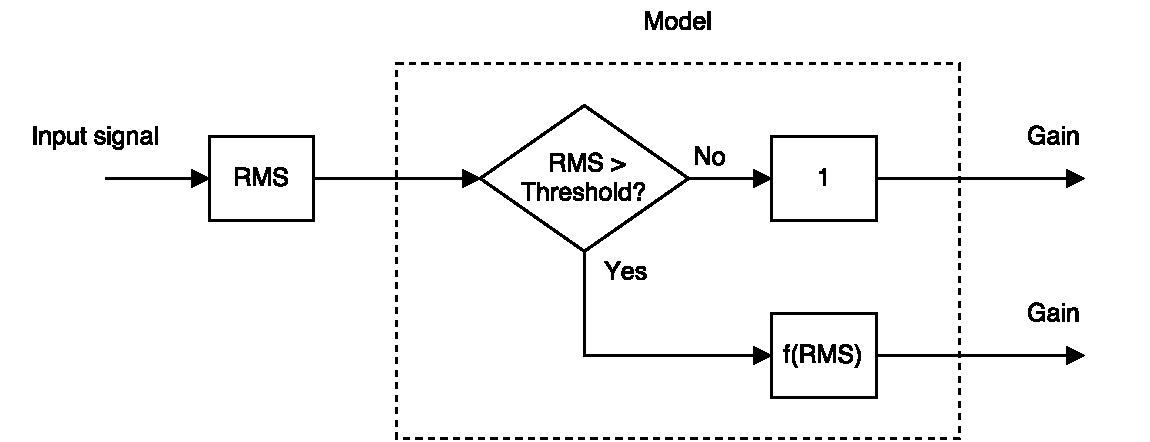
\includegraphics[width=\textwidth]{designRealRMS}
\end{figure}

%\begin{figure}
%	\centering
%	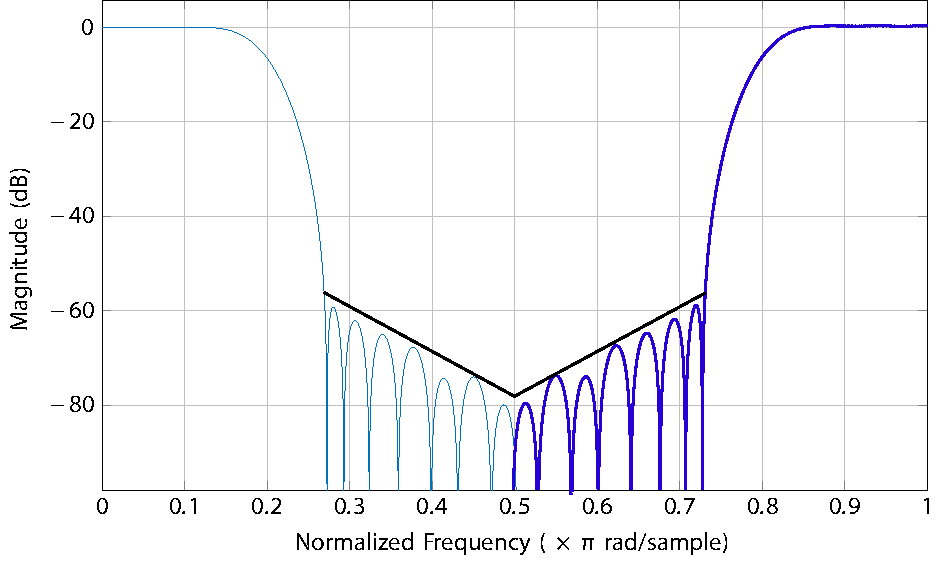
\includegraphics[width=0.8\textwidth]{DecIntCompMirror}
%\end{figure}

  \end{column}
\end{columns}
\end{frame}


\begin{frame}{Opbygning}{Løbende Gennemsnit}
\textbf{Krav:}
\begin{itemize}
\item[$\surd$] Løbende Gennemsnit
\begin{itemize}
\item Nødvendige samples: $n = \frac{fs}{f_{lowest}}$
\begin{itemize}
\item Band 1-4: $n = \frac{375 Hz}{30 Hz} = 12.5 \approx 16$
\item Band 5: $n = \frac{3000 Hz}{30 Hz} = 100 \approx 128$
\end{itemize}
\end{itemize}
\end{itemize}
\begin{figure}
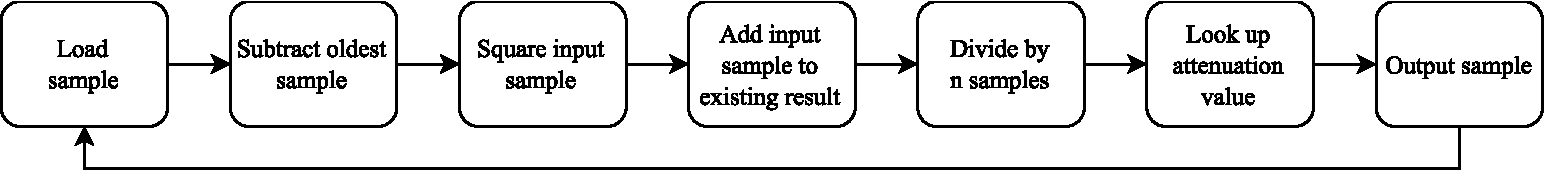
\includegraphics[width=1\textwidth]{Compressor}
\end{figure} 
\end{frame}


\begin{frame}{Opbygning}{Dæmpning til grænseværdi ved input på $\geq$ grænseværdien}
%\textbf{Krav:}
%\begin{itemize}
%\item[$\surd$] Løbende Gennemsnit
%\item \alert{Dæmpning til grænseværdi ved input på $\geq$ grænseværdien}
%\item 0 s attack time
%\item 5 s release time
%\end{itemize}
\begin{block}{Grænseværdier bestemmes ved at:}
Finde Maksimalt gennem hele systemet = 40 dB \\
Grænseværdien findes ved $\text{Threshold} = \frac{\sqrt{150 \text{W} \cdot 5 \Omega}}{100}=0.3 V$
\end{block}

\begin{block}{Look up tabellen laves:}
Opdele funktionen $\sqrt{\frac{Threshold^2}{RMS^2}}$ i 1024 steps \\

Beregn en Lookup tabel ved brug af formlen $\sqrt{\frac{\text{Threshold}^2}{(\frac{n}{1024})^2}}$
\end{block}
\begin{figure}
\centering
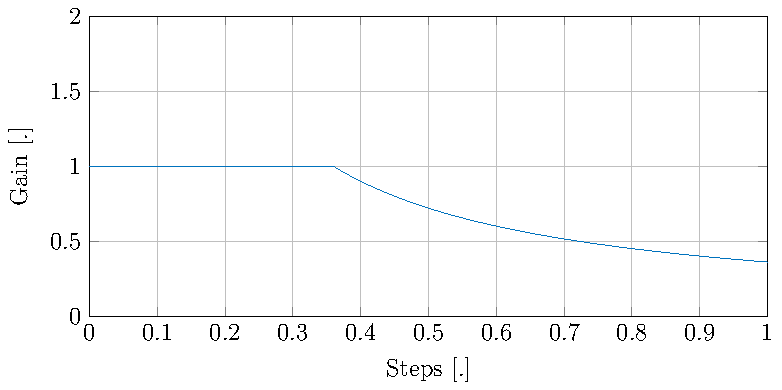
\includegraphics[width=0.5\textwidth]{LookUP}
\end{figure}



\end{frame}


\begin{frame}{Opbygning}{Attack \& Release time}
\begin{columns}
  \begin{column}{0.4\textwidth}
\textbf{Krav:}

\begin{itemize}
%\item[$\surd$] Løbende Gennemsnit
%\item[$\times$] \alert{Dæmpning til grænseværdi ved input på $\geq$ grænseværdien}
\item 0 s attack time
\begin{itemize}
\item Påfør gain med det samme
\end{itemize}
\item 5 s release time
\begin{itemize}
\item $H(s) = \frac{\omega_c}{s+\omega_c}$
\item $\tau = 5 \ s$
\begin{itemize}
\item $\omega_c=\frac{1}{\tau}$
\end{itemize}
\item $H(s) = \frac{0.2}{s+0.2}$
\end{itemize}
\item Impuls Invariant metode
\begin{itemize}
\item $H(s) = T\frac{0.2}{1-\text{e}^{-0.2T} z^{-1}}$
\end{itemize}
\end{itemize}

  \end{column}

  \begin{column}{0.6\textwidth}
\begin{figure}
\centering
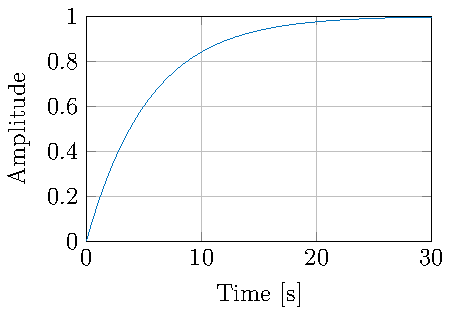
\includegraphics[width=0.7\textwidth]{releaseTimeDigitalStep}
\end{figure}

  \end{column}
\end{columns}
\end{frame}





















%%%%%%%%%%%%%%%%%%%%%%%%%%%%%%%%%%%%%%%%%%%%%%%%%%%%%%%%%%%%%%%%%%%%%%%%%%%%
%%%%%%%%%%%%%%%%%%%%%%%%%%%%%%%%%%%%%%%%%%%%%%%%%%%%%%%%%%%%%%%%%%%%%%%%%%%%
%%%%%%%%%%%%%%%%%%%%%%%%%%%%%%%%%%%%%%%%%%%%%%%%%%%%%%%%%%%%%%%%%%%%%%%%%%%%


\subsection{Interpolation}
\begin{frame}{Opbygning}{Interpolation}

\begin{columns}
  \begin{column}{0.4\textwidth}
%\begin{figure}
%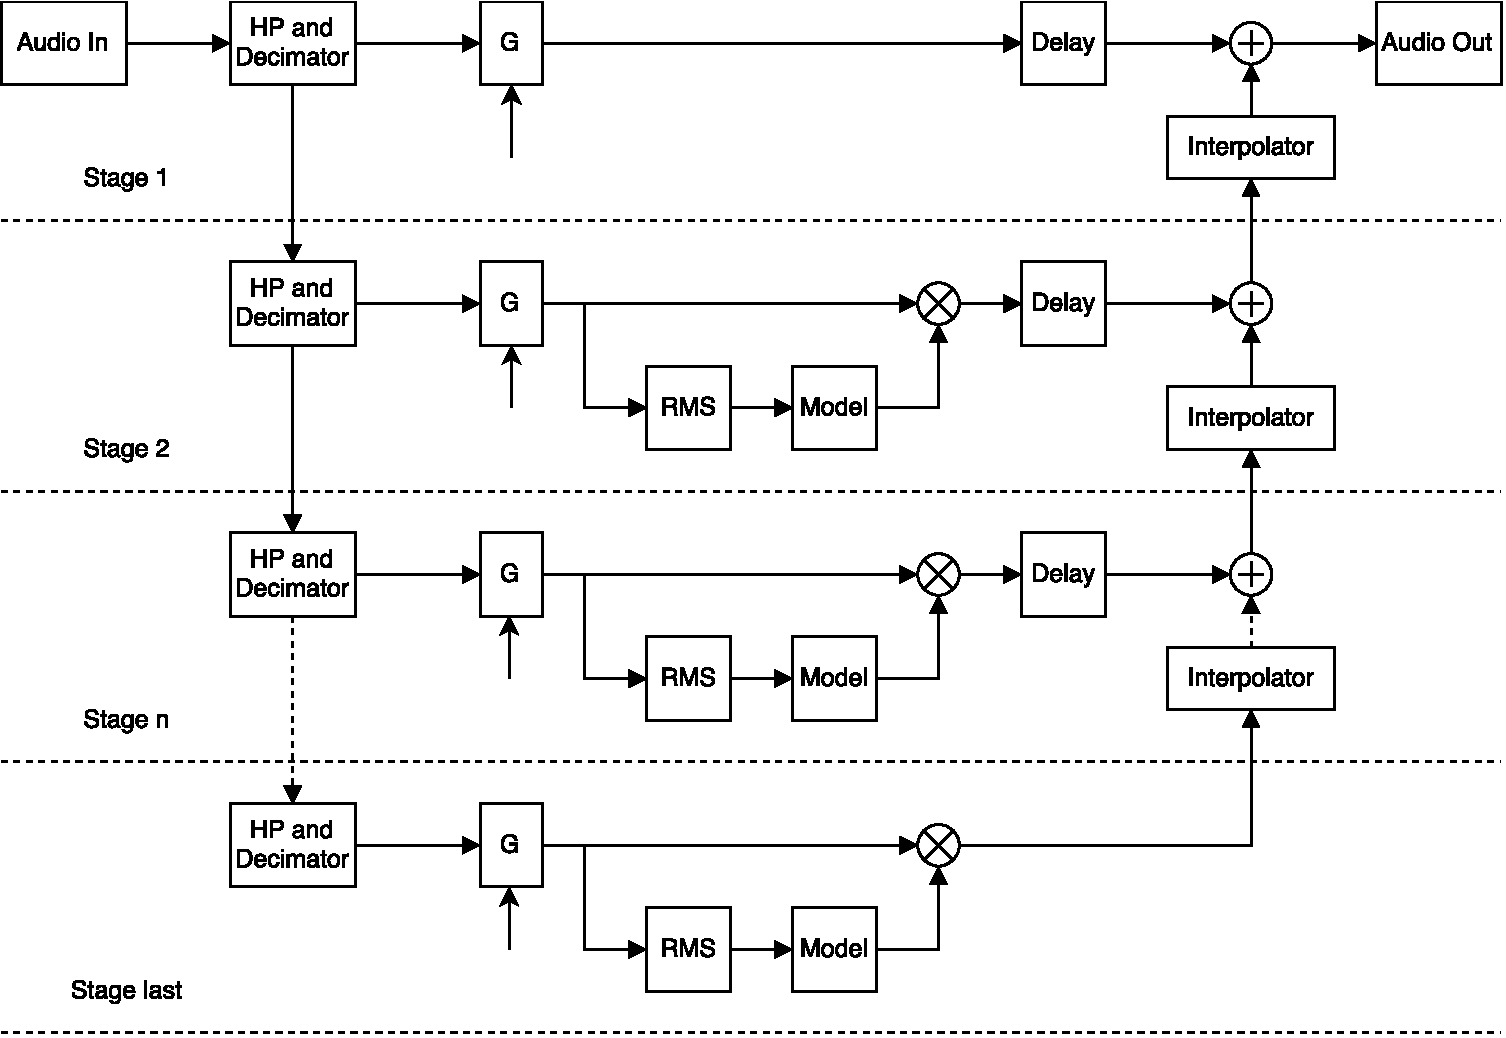
\includegraphics[width=0.9\textwidth]{designRealBlock1}
%\end{figure}
  \textbf{Funktionalitet:}
\begin{itemize}
\item Lavpas filter til rekonstruktion
\item Zero-padding til upsampling
\item Forstærkning med faktor $L$
\end{itemize}
\textbf{Krav:}
\begin{itemize}
\item Må ikke interfere med decimation filter bandwidth
\item \alert{60 dB dæmpning ved $\frac{fs}{2L}$}
\end{itemize}
  \end{column}

  \begin{column}{0.6\textwidth}
\begin{figure}
\centering
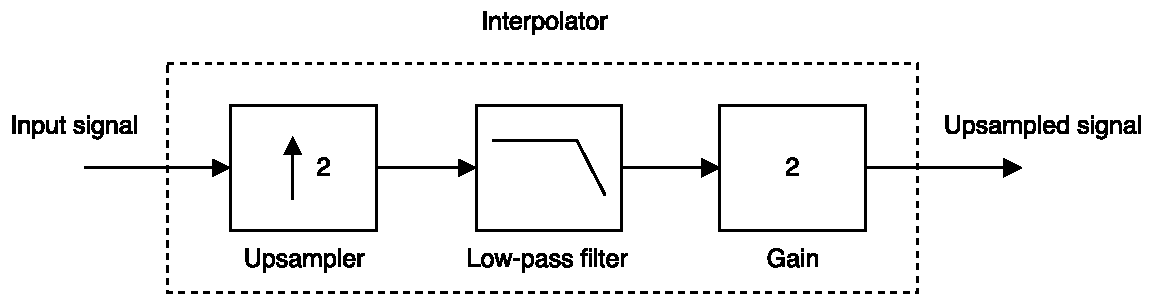
\includegraphics[width=\textwidth]{designRealInterpolator}
\end{figure}

%\begin{figure}
%	\centering
%	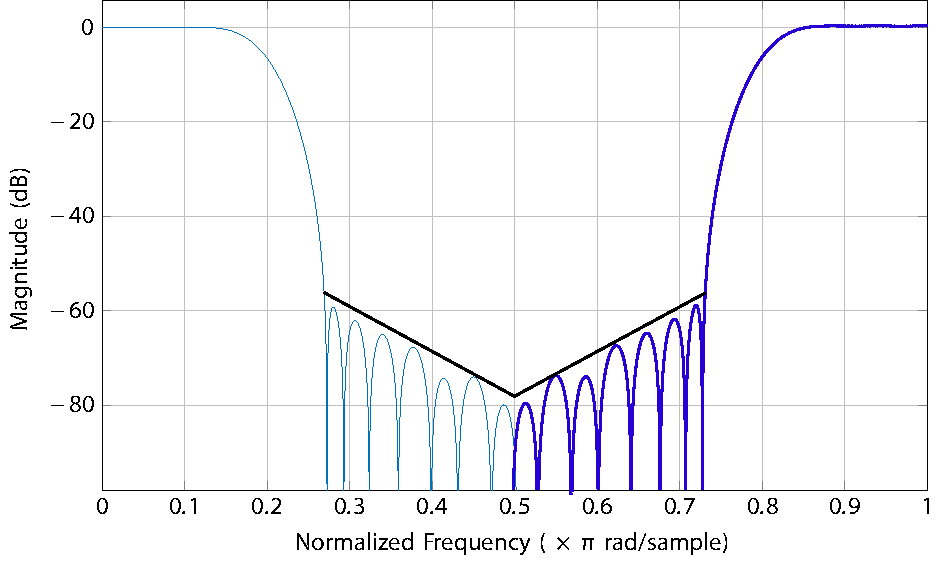
\includegraphics[width=0.8\textwidth]{DecIntCompMirror}
%\end{figure}

  \end{column}
\end{columns}

\end{frame}

\begin{frame}{Opbygning}{Må ikke interfere med decimation filter bandwidth}
\begin{columns}
  \begin{column}{0.4\textwidth}
%\begin{figure}
%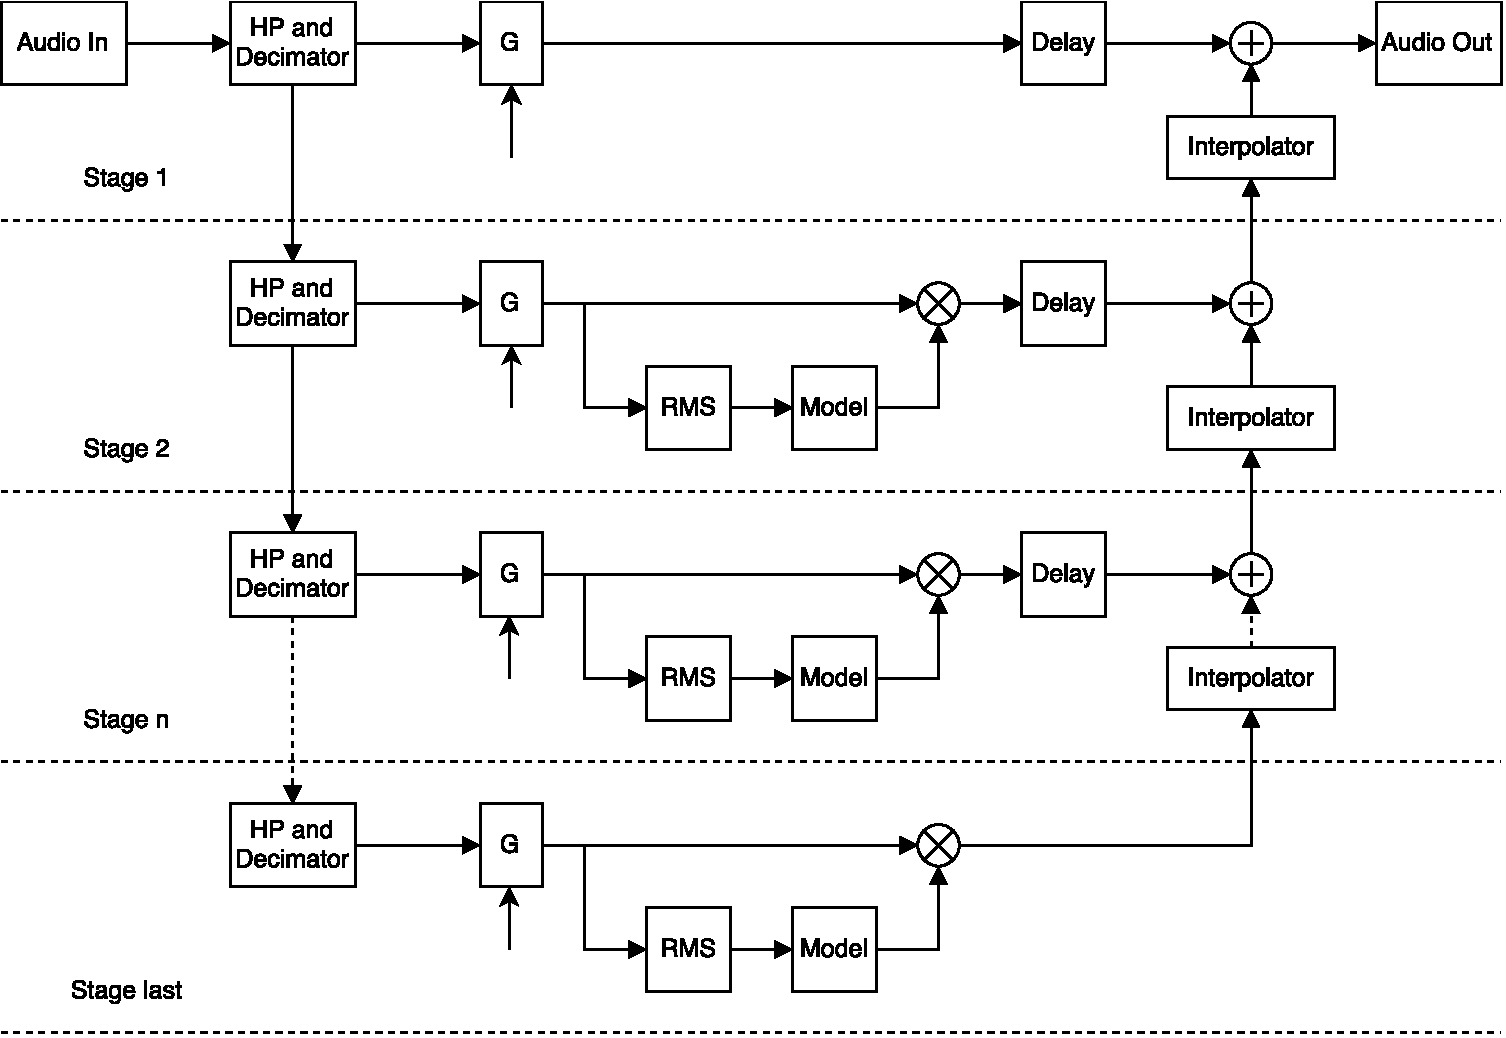
\includegraphics[width=0.9\textwidth]{designRealBlock1}
%\end{figure}
%  \textbf{Funktionalitet:}
%\begin{itemize}
%\item Lavpas filter til rekonstruktion
%\item Zero-padding til upsampling
%\item Forstærkning med faktor $L$
%\end{itemize}
\textbf{Krav:}
\begin{itemize}
\item Må ikke interfere med decimation filter bandwidth
\begin{itemize}
\item over 0.3 $\frac{\pi rad}{sample}$
\item under 0.7 $\frac{\pi rad}{sample}$
\end{itemize}
\item \alert{60 dB dæmpning ved $\frac{fs}{2L}$}
\end{itemize}
  \end{column}
  \begin{column}{0.6\textwidth}
%\begin{figure}
%\centering
%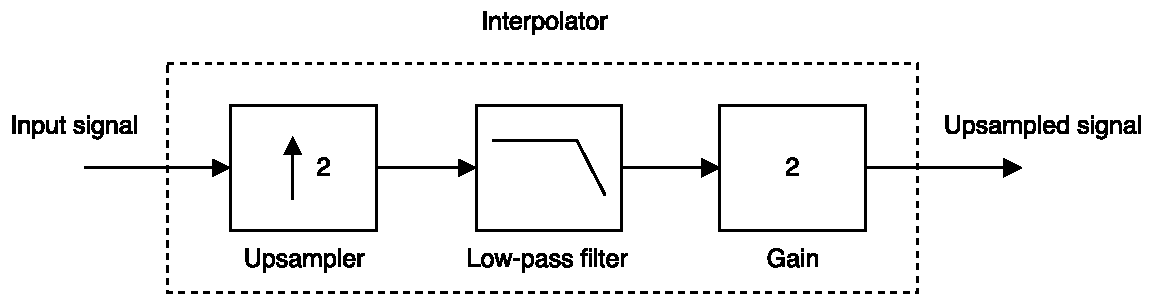
\includegraphics[width=\textwidth]{designRealInterpolator}
%\end{figure}
\begin{figure}
	\centering
	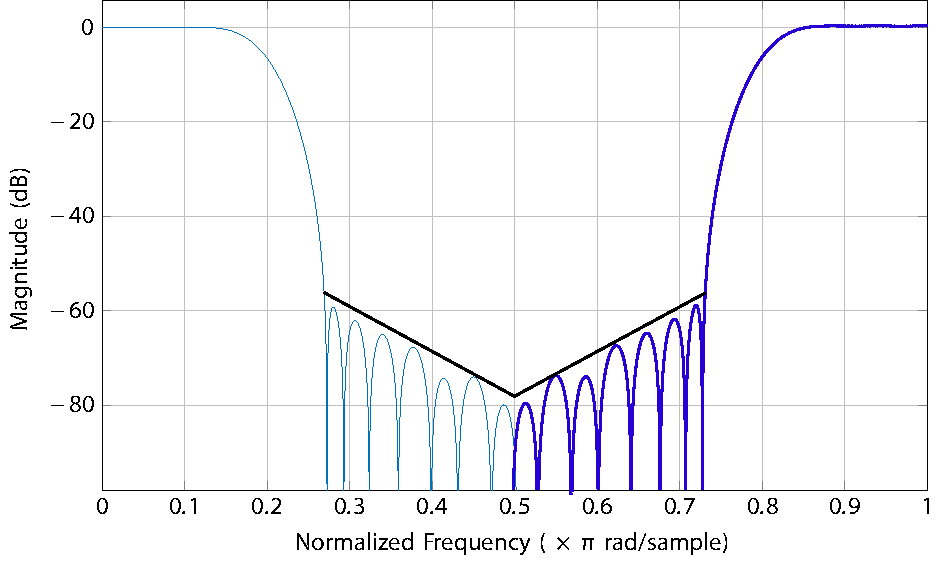
\includegraphics[width=1\textwidth]{DecIntCompMirror}
\end{figure}
  \end{column}
\end{columns}
\end{frame}

\begin{frame}{Opbygning}{60 dB dæmpning ved $\frac{fs}{2L}$}
\begin{columns}
  \begin{column}{0.4\textwidth}
%\begin{figure}
%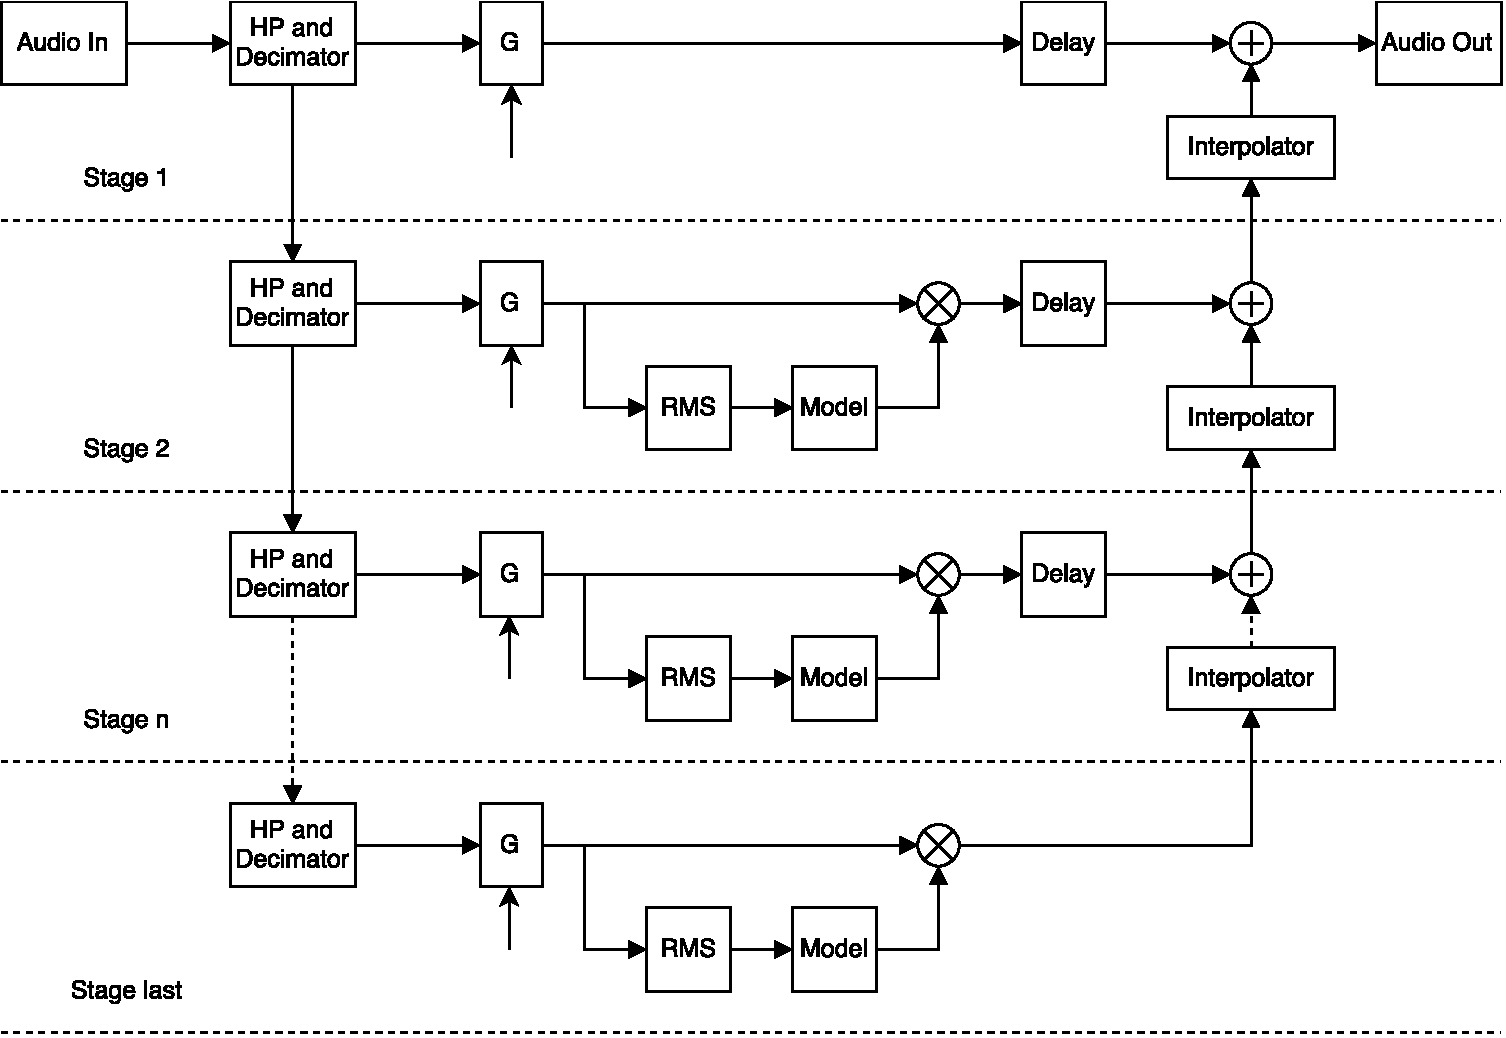
\includegraphics[width=0.9\textwidth]{designRealBlock1}
%\end{figure}
%  \textbf{Funktionalitet:}
%\begin{itemize}
%\item Lavpas filter til rekonstruktion
%\item Zero-padding til upsampling
%\item Forstærkning med faktor $L$
%\end{itemize}
\textbf{Krav:}
\begin{itemize}
\item[$\surd$] Må ikke interfere med decimation filter bandwidth
\item[$\surd$] \alert{60 dB dæmpning ved $\frac{fs}{2L}$}
\begin{itemize}
\item 34. Orden FIR
\item Type 1
\end{itemize}
\end{itemize}
  \end{column}
  \begin{column}{0.6\textwidth}
%\begin{figure}
%\centering
%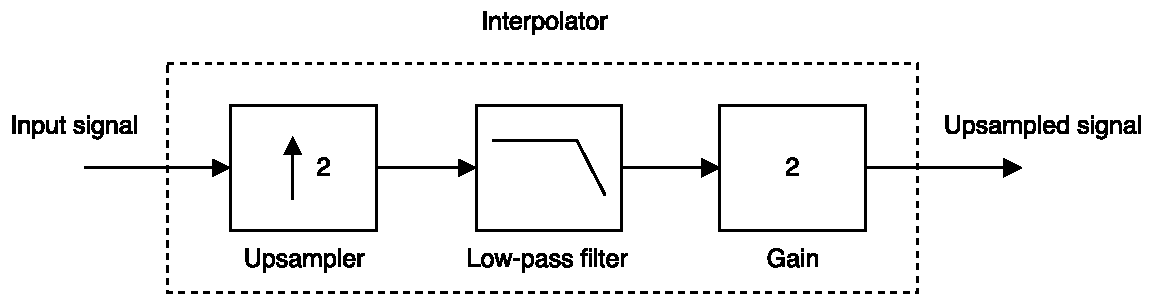
\includegraphics[width=\textwidth]{designRealInterpolator}
%\end{figure}
\begin{figure}
	\centering
	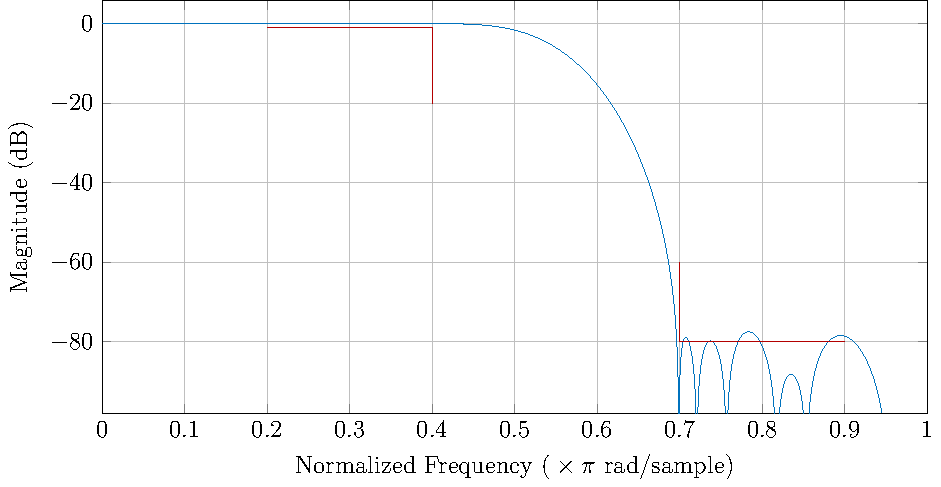
\includegraphics[width=1\textwidth]{IntMag}
\end{figure}
  \end{column}
\end{columns}
\end{frame}